\section{stockert}
\begin{frame}{Messung am Stockert}
  \begin{columns}[c, onlytextwidth]
    \begin{column}{0.4\textwidth}
      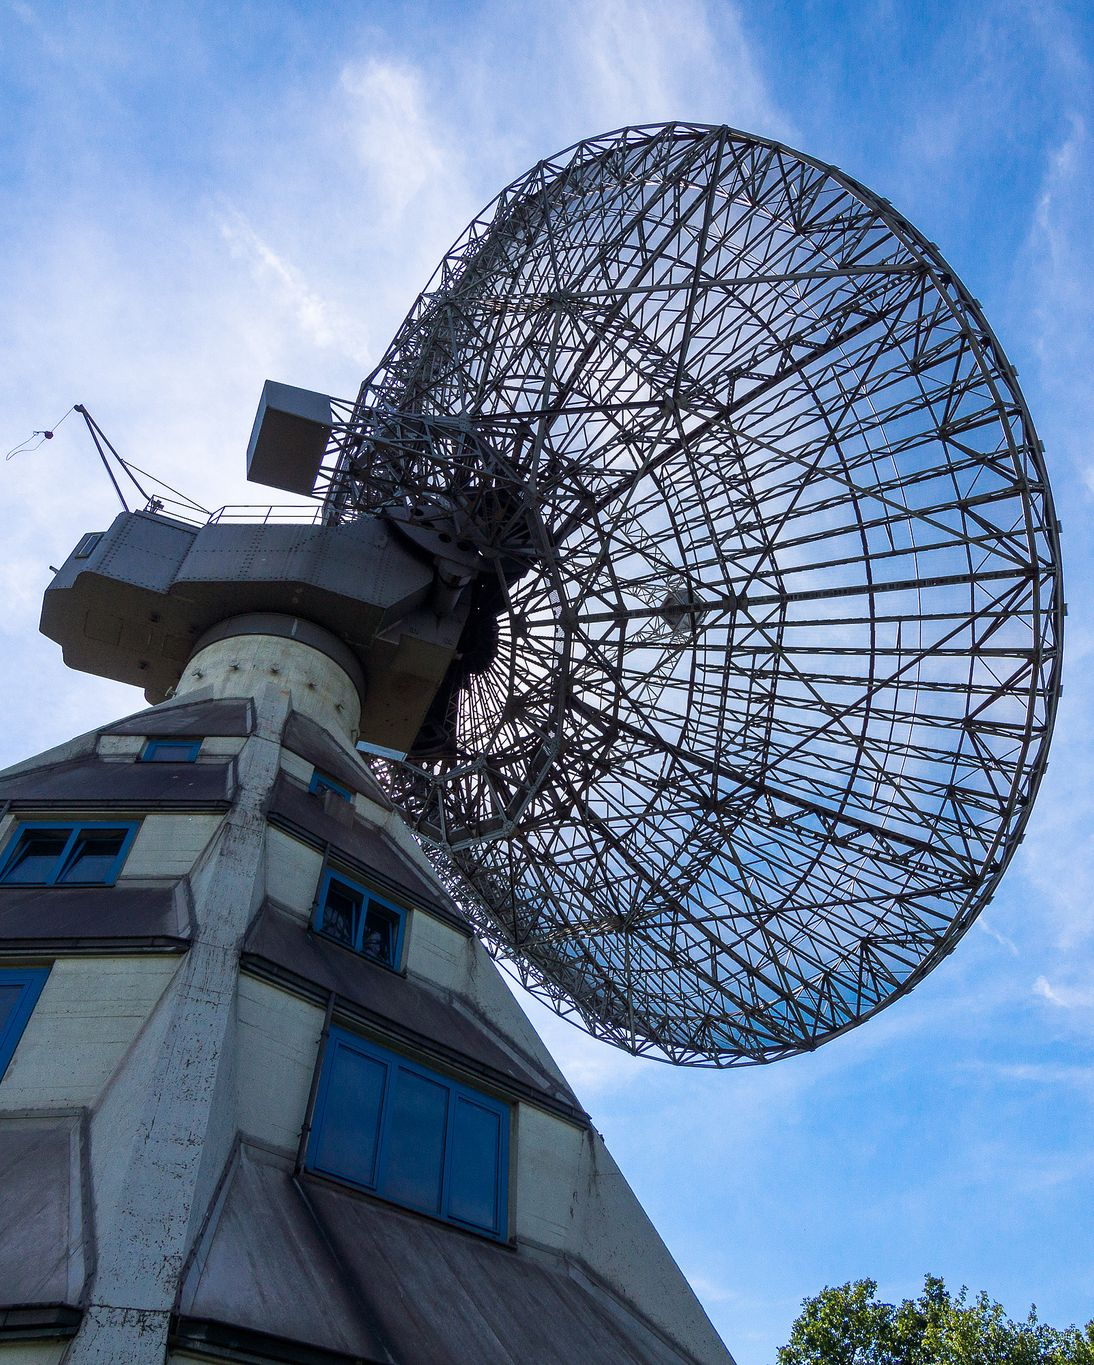
\includegraphics[width=\linewidth]{images/stockert_crop.jpg}
    \end{column}
    \begin{column}{0.55\textwidth}
      \begin{description}[Durchmesser]
        \item[Baujahr] 1956
        \item[Durchmesser] \SI{25}{\meter}
        \item[Auflösung]  \SI{0.5}{\degree} FWHM für $λ = \SI{21}{\centi\meter}$
      \end{description}
    \end{column}
  \end{columns}
\end{frame}
